\section{Arsitektur Sistem Operasi Linux}
\subsection{Kernel}
	Kernel Linux merupakan kernel yang digunakan dalam sistem operasi GNU/Linux. Kernel ini merupakan turunan dari sistem operasi UNIX, yang mana di rilis menggunakan lisensi GNU \textit{General Public License} (GPL) dan dikembangkan oleh programmer di selururh dunia karena sifatnya yang \textit{open source}. Kernel ini merupakan inti dari sistem operasi komputer dengan memiliki kontrol penuh atas segala dalam sistem tersebut. Kernel ini menghubungkan antara perangkat lunak dan perangkat keras seperti pada gambar \textbf{\ref{kernel}}, salah satu program pertama yang memuat fungsi kernel ini yaitu dimuat didalam start-up setelah proses bootloader.

\begin{figure}[!htbp]
\centerline{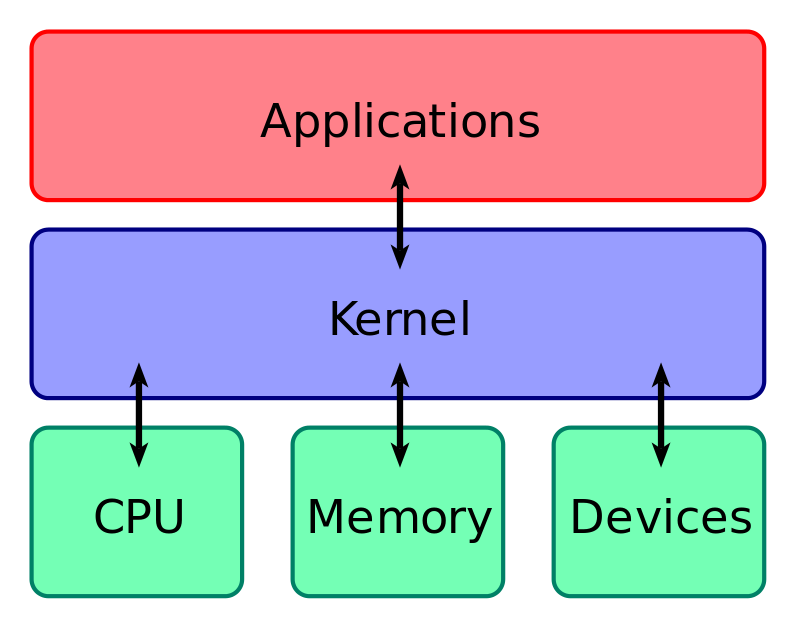
\includegraphics[width=0.75\textwidth]{Figures/Kernel_Layout.png}}
\caption{Kernel connect}
\label{kernel}
\end{figure}

\lstinputlisting[caption=contoh dasar kode program kerne membuat hello world,label={lst:kode dasar}]{src/contoh.tex}

\subsection{struktur data kernel}
	Ketika kernel melakukan sebuah proses, data-data proses tersebut akan disimpan secara periodik ke dalam bentuk file-file. Untuk dapat melihat data kernel, maka file-file tersebut harus diparsing setiap saat dikarenakan datanya yang dinamis \cite{raharja2001pengenalan}. Cara termudah untuk melakukan hal tersebut yaitu menggunakan perintah \textbf{cat} \ref{lst:kode dasar2}

\lstinputlisting[caption=Perintah cat pada linux,label={lst:kode dasar2}]{src/cat.sh}
File-file ini akan tersimpan di dalam direktori yang tersetruktur dalam direktori /proc.

\subsection{Instalasi}
Setelah kita memahami tentang kernel dan juga struktur data kernel, selanjutnya kita akan mencoba install kernel sebelum itu kita dapat cek versi kernel kita dengan mengetikan pada terminal 
\begin{verbatim}
$ uname -r 
\end{verbatim}
\textbf{uname} ini merupakan perintah untuk mengetahui sistem informasi dan \textbf{-r} merupakan perintah untuk menampilkan versi kernel.
 
Untuk instalasi sendiri terdapat beberapa cara yaitu kamu bisa mendownload package dan mencompile dari sumber atau bisa juga hasil download package management tools.
dengan mengetikan pada terminal
\begin{verbatim}
$ sudo apt install linux-generic-lts-vivid
\end{verbatim}
 sebagai contoh : \textbf{sudo apt install 3.19.0-43-generic} setelah itu tinggal reboot maka kernel yang kita compile tadi akan terinstall.
cara alternatif selain itu kita dapat langsung meng-\textit{upgrade} versi kernel dengan menggunakan \textbf{dist-upgrade} maka itu akan mengupdate semua package di dalam sistem. 
 \begin{verbatim}
$ sudo apt dist-upgrade
\end{verbatim}

Setelah melakukan penginstalan sebuah kernel, maka itu akan menambah beberapa file system yang ditambahkan di direktori /boot
kamu akan mendapatkan beberapa file untuk versi kernel yang berbeda seperti :
\begin{enumerate}
\item \textbf{vmlinuz} - ini adalah kernel linux yang sebenarnya
\item \textbf{initrd} - ini digunakan sebagai sistem berkas sementara sebelum memuat kernel
\item \textbf{system.map} - ini sebagai table simbol 
\item \textbf{config} - ini sebagai pengaturan kernel, jika kamu mencompile kernel sendiri maka kamu dapat mengatur modul-modul yang dimuat
\end{enumerate}
Ketika direktori /boot kehabisan ruang penyimpanan, kamu dapat menghapus versi lama dari file-file atau package yang lama. Tapi harus berhati-hati ketika melakukan pemeliharaan di dalam direktori ini karena ditakutkan akan menghapus kernel yang digunakan secara tidak sengaja.